\documentclass{maine-thesis}  % Default options 12pt and final copy
\usepackage{amsthm, amssymb, amsmath}
\usepackage{mathtools}
\usepackage{indentfirst}
\usepackage{array}
\usepackage{graphicx}
\usepackage{caption}
\usepackage[left=1.5in, top = 1in, right = 1in, bottom=1in]{geometry}
\usepackage{multicol}
\usepackage{url}
\usepackage{hyperref}
\usepackage{natbib}
\usepackage{etoolbox}


%%%%%%%%%%%%%%%%%%%%%%%%%%%%%%%%%%%%%%%%%%%%%%%%
% Preamble definitions and general formatting
\def\BibTeX{{\rm B\kern-.05em{\sc i\kern-.025em b}\kern-.08em
    T\kern-.1667em\lower.7ex\hbox{E}\kern-.125emX}}

\setlength\parindent{20pt}
%%%%%%%%%%%%%%%%%%%%%%%%%%%%%%%%%%%%%%%%%%%%%%%%

% Replace contents of {...} with your own information.
\title{TITLE FOR GRADUATE THESIS \LaTeX TEMPLATE \protect\\ IS IN ALL CAPS WITH DOWNWARD  \protect\\ INVERTED TRIANGLE}					% Title of thesis
\author{Ian McKee Nesbitt}					% Author's name: First Middle Last
\degreesheld{B.A. Williams College, 2013}			% Previously earned degree(s), institution(s) and year(s).  
\degree{Master of Science}  				% Degree to be granted
\program{Earth and Climate Sciences}				% Degree granting department or program
\submitdate{Month YYYY}				% Month and year of graduation (do not separate with a comma)

\principaladvisor{Seth William Campbell, Research Assistant Professor} 			% Advisors name, title
% If you have more than one advisor then you'll also need the following command, otherwise comment out or delete it
% \secondadvisor{...}

% Include all committee members names and titles
\firstreader{Sean M.C. Smith, Associate Professor}        
\secondreader{Katherine A. Allen, Assistant Professor}
% If necessary (i.e. for a doctorate), include extra committee members.  Else, comment out or delete any that are unnecessary
% \thirdreader{...}
% \fourthreader{...}
% \fifthreader{...}

\principalshort{Campbell} 			% Shortened advisor name for abstract (last name).  See guidelines for example.
								 
% If the thesis has MORE than one appendix, leave the following command in.  Else, comment it out.
\multipleappendicestrue 

% Begin the document.
\begin{document}
\preliminary
\titlepage

%%%%%%%%%%%%%%%%%%%%%%%%%%%%%%%%%%%%%%%%%%%%%%%%%%%%%%%%%%%%%%%%%%%%%%%%%%%%%%
%\copyrightpage[...]{...}		% Optional, comment out or delete if undesired

\begin{abstract}

This is the abstract. Sentence two. Formatting is easy when you use \LaTeX\ and it's easy to control. It excels in the math environement but tables can sometimes require more effort. Fortunately, it's open source (i.e. free), platform independent, and there's a big user community. There's a list of resources at the end.


\end{abstract}

%\begin{layabstract}{...}	% Replace the ... with the list of keywords
% Lay abstract text here, either typed in directly or included using an `\input{}' command
%\end{layabstract}

% The optional preface, dedication, and acknowledgements environments are included similar to the abstract environment

%%%%%%%%%%%%%%%%%%%%%%%%%%%% Preface %%%%%%%%%%%%%%%%%%%%%%%%%%%%%%%%%
%\begin{preface}
% Preface text here
%\end{preface} 

%%%%%%%%%%%%%%%%%%%%%%%%%%% Dedication %%%%%%%%%%%%%%%%%%%%%%%%%%%%%%%
%\begin{dedication}
% Dedication text here
%\end{dedication}

%%%%%%%%%%%%%%%%%%%%%%%% Acknowledgements %%%%%%%%%%%%%%%%%%%%%%%%%%%%
%\begin{acknowledgements}
% Acknowledgments text here
%\end{acknowledgements}


%%%%%%%%%%%%%%%%%%%%%%%%%%%%%%%%%%%%%%%%%%%%%%%%%%%%%%%%%%%%%%%%%%%%%%
% Commands for the required lists
\setcounter{page}{2}
\tableofcontents
\listoftables				% Include only if there are tables in the thesis
\listoffigures				% Include only if there are figures in the thesis


%%%%%%%%%%%%%%%%%%%%%%%%%%%%%%%%%%%%%%%%%%%%%%%%%%%%%%%%%%%%%%%%%%%%%%
%% For a section that needs to be included in the front matter insert into PreChapter.tex file. 
\newpage
\addcontentsline{toc}{chapter}{Front Matter Chapter}

% Abbreviations and such need to be in the front matter. The numbering needs to be roman numerals
\begin{center}
\textbf{LIST OF ABBREVIATIONS}
\end{center}
\begin{multicols}{2}
\noindent 2D - Two-Dimensional\\
\noindent 3D - Three-Dimensional\\
\noindent DEM - Digital Elevation Model\\
\noindent DSLR - Digital Single Lens Reflex\\
\noindent GCP - Ground Control Point\\
\noindent GeoTIFF - Georeferenced Tagged Image File Format\\
\noindent GIS - Geographical Information System\\
\noindent GPR - Ground-Penetrating Radar\\
\noindent GPS - Global Positioning System\\
\noindent GSSI - Geophysical Survey Systems Incorporated\\
\noindent IMU - Inertial Measurement Unit\\
\noindent LIA - Little Ice Age\\
\noindent LiDAR - Light Detection And Ranging\\
\noindent LIS - Laurentide Ice Sheet\\
\noindent m.a.s.l. - Meters Above Mean Sea Level\\
\noindent MTL - Marine Transgression Line\\
\noindent radar - Radio Detection And Ranging\\
\noindent RGB - Red, Green, Blue\\
\noindent RMS - Root Mean Square\\
\noindent RTK - Real Time Kinematic\\
\noindent SfM - Structure from Motion\\
\noindent SLR - Sea Level Rise\\
\noindent SSS - Sidescan Sonar\\
\noindent w.e. - Water Equivalent\\
\end{multicols}
\endinput

% If you have other lists which need to be included they go here, possibly using the listof environment
%\begin{listof}{...}		% Replace the ... with name of the things being listed here
% Contents of list
%\end{listof}

% Sets the document spacing and pagestyle.  It is recommended that the `bottom' option be used. 
\mainmatter{bottom} 	

\endinput

%%%%%%%%%%%%%%%%%%%%%%%%%%%%%%%%% Body %%%%%%%%%%%%%%%%%%%%%%%%%%%%%%%%%%%%%%%
% Main text of the thesis.  Use of the `\input' command will make later editing much easier.

\chapter{Introduction}	%Chapter title


\endinput				
\chapter{Methods}

To refer to a table use \ref{tab::comparison}. When labeling the table, put the label after you end the tabular environment.

\begin{table}
\caption{Example table from some data$^\dagger$.}
\centering 
\begin{tabular}{l m{2.2cm} m{2.2cm} m{2.2cm} c m{1.8cm}}
\hline 
\textbf{{Point}} & \textbf{Elevation GPS '99} & \textbf{2015 Pixel Elev} & \textbf{Diff 1999-Raster} & \textbf{Ratio} & \textbf{Ratio (no outlier)} \\ 
\hline
99-1a &				1621.055 & 842.0439 & 779.011  & 1.93 & 1.93\\[0.2cm]
99-3a-1 &			1891.129 & 1008.286 & 882.843  & 1.88 & 1.88 \\[0.2cm]
Ed Little [99-3b] &	1885.780 & 1048.884 & 836.896  & 1.80 & \\[0.2cm]
99-4a &				1830.979 & 999.385  & 831.594  & 1.83 & 1.83\\[0.2cm]
C29-1a &			1611.290 & 828.326  & 782.964  & 1.95 & 1.95\\[0.2cm]
C29-1b &			1611.895 & 831.478  & 780.417  & 1.94 & 1.94\\[0.2cm]
C29-1c &			1611.391 & 830.311  & 781.599  & 1.94 & 1.94\\[0.2cm]
C29-3 &				1611.177 & 831.162  & 780.015  & 1.94 & 1.94\\[0.2cm]
C29 Tripod &		1611.247 & 820.626  & 790.621  & 1.96 & 1.96\\[0.2cm]
Cathedral Peak &	2134.177 & 1113.373 & 1020.804 & 1.92 & 1.92\\[0.2cm]
Generator 2 &		1613.978 & 829.450  & 784.528  & 1.95 & 1.95\\[0.2cm]
Lower Cirque &		2060.727 & 1074.479 & 986.248  & 1.92 & 1.92\\[0.2cm]
Metal Marker &		1602.020 & 792.410  & 809.610  & 2.02 & \\[0.2cm]
FFGR 75 &			1610.663 & 820.620  & 790.043  & 1.96 & 1.96 \\[0.2cm]
\hline 
\multicolumn{3}{r}{\textbf{Average}} 	& 831.228 & 1.923 & 1.925 \\[0.2cm]
\multicolumn{3}{r}{\textbf{Std Dev}} 			& 79.122 & 0.056 & 0.038 \\[0.2cm]
\multicolumn{3}{r}{\textbf{Error}} (\%) 			& 9.5 & 2.9 & 2.0 \\[0.2cm]
\hline
\multicolumn{6}{p{15cm} }{\footnotesize$^\dagger$Using the ratio of the values of the 1999 GCP elevation to the nearby pixel values of the 2015 SfM DEM results in a scalar that has a better fit than using a simple difference, and removing the outliers lowers the variation by a third while only changing the scalar by 0.1\%.}
\end{tabular}
\label{tab::comparison}
\end{table}

For an equation we have 
\begin{equation}
	A = \pi r^2
\end{equation}
but a more fun equation is
\begin{equation}
	\nabla^2 x = \frac{d^2 u}{d t^2}.
    \label{eq::wave}
\end{equation}
Referencing equation is easy and you can label it at the end of the equation environment. Eq. (\ref{eq::wave}) is the wave equation. Equations can be entered in-line using the \$ symbol to start and end an in-line math equation. For example, $\sigma_{ij} = \lambda \varepsilon_{kk} \delta_{ij} + \mu \varepsilon_{ij} $. 

%%%%%%%%%%%%%%%%%%%%%%%%%%%%%%%%%%%%%%%%%%%%%%%%%%%%%%%%%%%%%%%%%%%%%%%%%%%%%%%%

Referring to figures is easy too. Check out Fig \ref{fig::easy} 

\begin{figure}[!ht]
	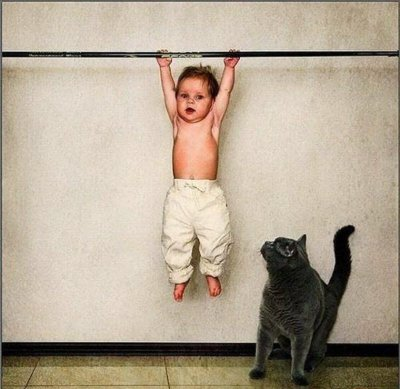
\includegraphics[width=0.8\textwidth]{babydoingpullups}
    \caption{How hard can it be if a baby can do it?}
    \label{fig::easy}
\end{figure}

If you need help, there is a lot of help topics in for form of online forums and wiki's. A google search of your formatting problems is a good start but here's a list of some resources to get started if you're new at \LaTeX:

\begin{itemize}
	\item \url{http://www.sharelatex.com} - Documentation and general help
    \item \url{http://www.overleaf.com} - Free online \LaTeX environment that has a word count function for the times when you're doing the bare minimum 
    \item \url{https://stackoverflow.com} - Answers to \LaTeX questions and all of your other homework questions. 
    \item \url{reu.dimacs.rutgers.edu/Symbols.pdf} - a cheat sheet for the math environment.
    \item \url{http://www.bibtex.org/} - Help for using \BibTeX. Mendeley, Zotero and a few other reference managers have \BibTeX support and can be linked easily. 
\end{itemize}


\endinput				
%\chapter{Results}

\endinput				
%\chapter{The title of the 4th chapter}

\endinput


%%%%%%%%%%%%%%%%%%%%%%% References and Appendices %%%%%%%%%%%%%%%%%%%%%%%%%%%%
% Inserts and formats the reference section.

% Bibliography files are included here.  Separate with a comma if more than one
\addcontentsline{toc}{chapter}{REFERENCES}

% The included .sty file is the American Geophysical Union format. Most organizations have a .sty file from their website
\bibliographystyle{agufull08} 		

% Set single space bib entries and double space between entries
\begingroup
\setlength{\bibsep}{12pt}
\linespread{1}\selectfont 
% Create a Master Reference list. Only those cited will show up in the references
\bibliography{skeleton/MASTERS}
\endgroup

\appendix					% Include this before any appendices.
\chapter{...}	%Appendix title

\endinput				% First appendix.
%\chapter{...}	%Appendix title

\endinput				% Second appendix, etc.

\begin{biography}			% Biography of the author
Ian Nesbitt was born in North Adams, MA, on November 12, 1990. He attended Mount Greylock Regional High School and Holderness School, where he graduated in 2009. In June 2013, he received a B.A. with honors in geosciences from Williams College, where he also competed as a NCAA Division I Nordic skier. At his previous workplace, he oversaw the field side of large geophysical projects for a small company in southwestern Connecticut. The job taught him many things, including  surveying, piloting, and seamanship of small (~60 foot, 50 ton) vessels in the crowded waters of the lower Hudson and East Rivers. Ian grew up on pine cobble
\end{biography}

\endinput

\end{document}
